\section{Motivation}\label{sec:motivation}
This section introduces the motivation for this work, which aims to address effective root cause localization by jointly integrating an accurate anomaly detector and being driven by multi-source monitoring data.
The examples are taken from data collected from a benchmark microservice system, TrainTicket~\cite{TrainTicket}. Details about data collection will be introduced in~\cref{sec:data}.

\subsection{Can different sources of data besides traces be helpful?}\label{sec:study:multi-source}
We find that \textit{traces are insufficient to reveal all potential faults despite their wide usage.}
Most, if not all, previous related works~\cite{Trace17, TraceAnomaly, TraceRCA, MMTrace, MicroCause, MicroScope, MicroRank} are trace-based, indicating traces are informative and valuable.
However, traces focus on recording interactions between microservices and provide a holistic view of the system in practice.
Such high-level information only enables basic queries for coarse-grained information rather than intra-service information. 
For example, latency or error rate in traces can suggest a microservice's availability, yet fine-grained information like memory usage reflecting the intra-service status is unknowable.
%%%%% Latency is useful but not sufficient
This is consistent with our observation that latency is sensitive to network-related issues but cannot adequately reflect resource exhaustion-related anomalies.
Figure~\ref{fig:travel-latency} shows an example where a point denotes an invocation taking the microservice ``travel'' as the callee.
When Network Jam or Packet Loss is injected, the latency is abnormally high (marked with stars), but the latency during the CPU exhaustion injection period does not display obviously abnormal patterns. 
This case reminds us to be careful of relying on traces only. 
Since traces are informative but cannot reveal all anomalies, trace-based methods may omit potential failures. We need extra information to mitigate the anomaly omission problem.

\begin{figure}[htb]
    \centering
    \vspace{-0.1in}
        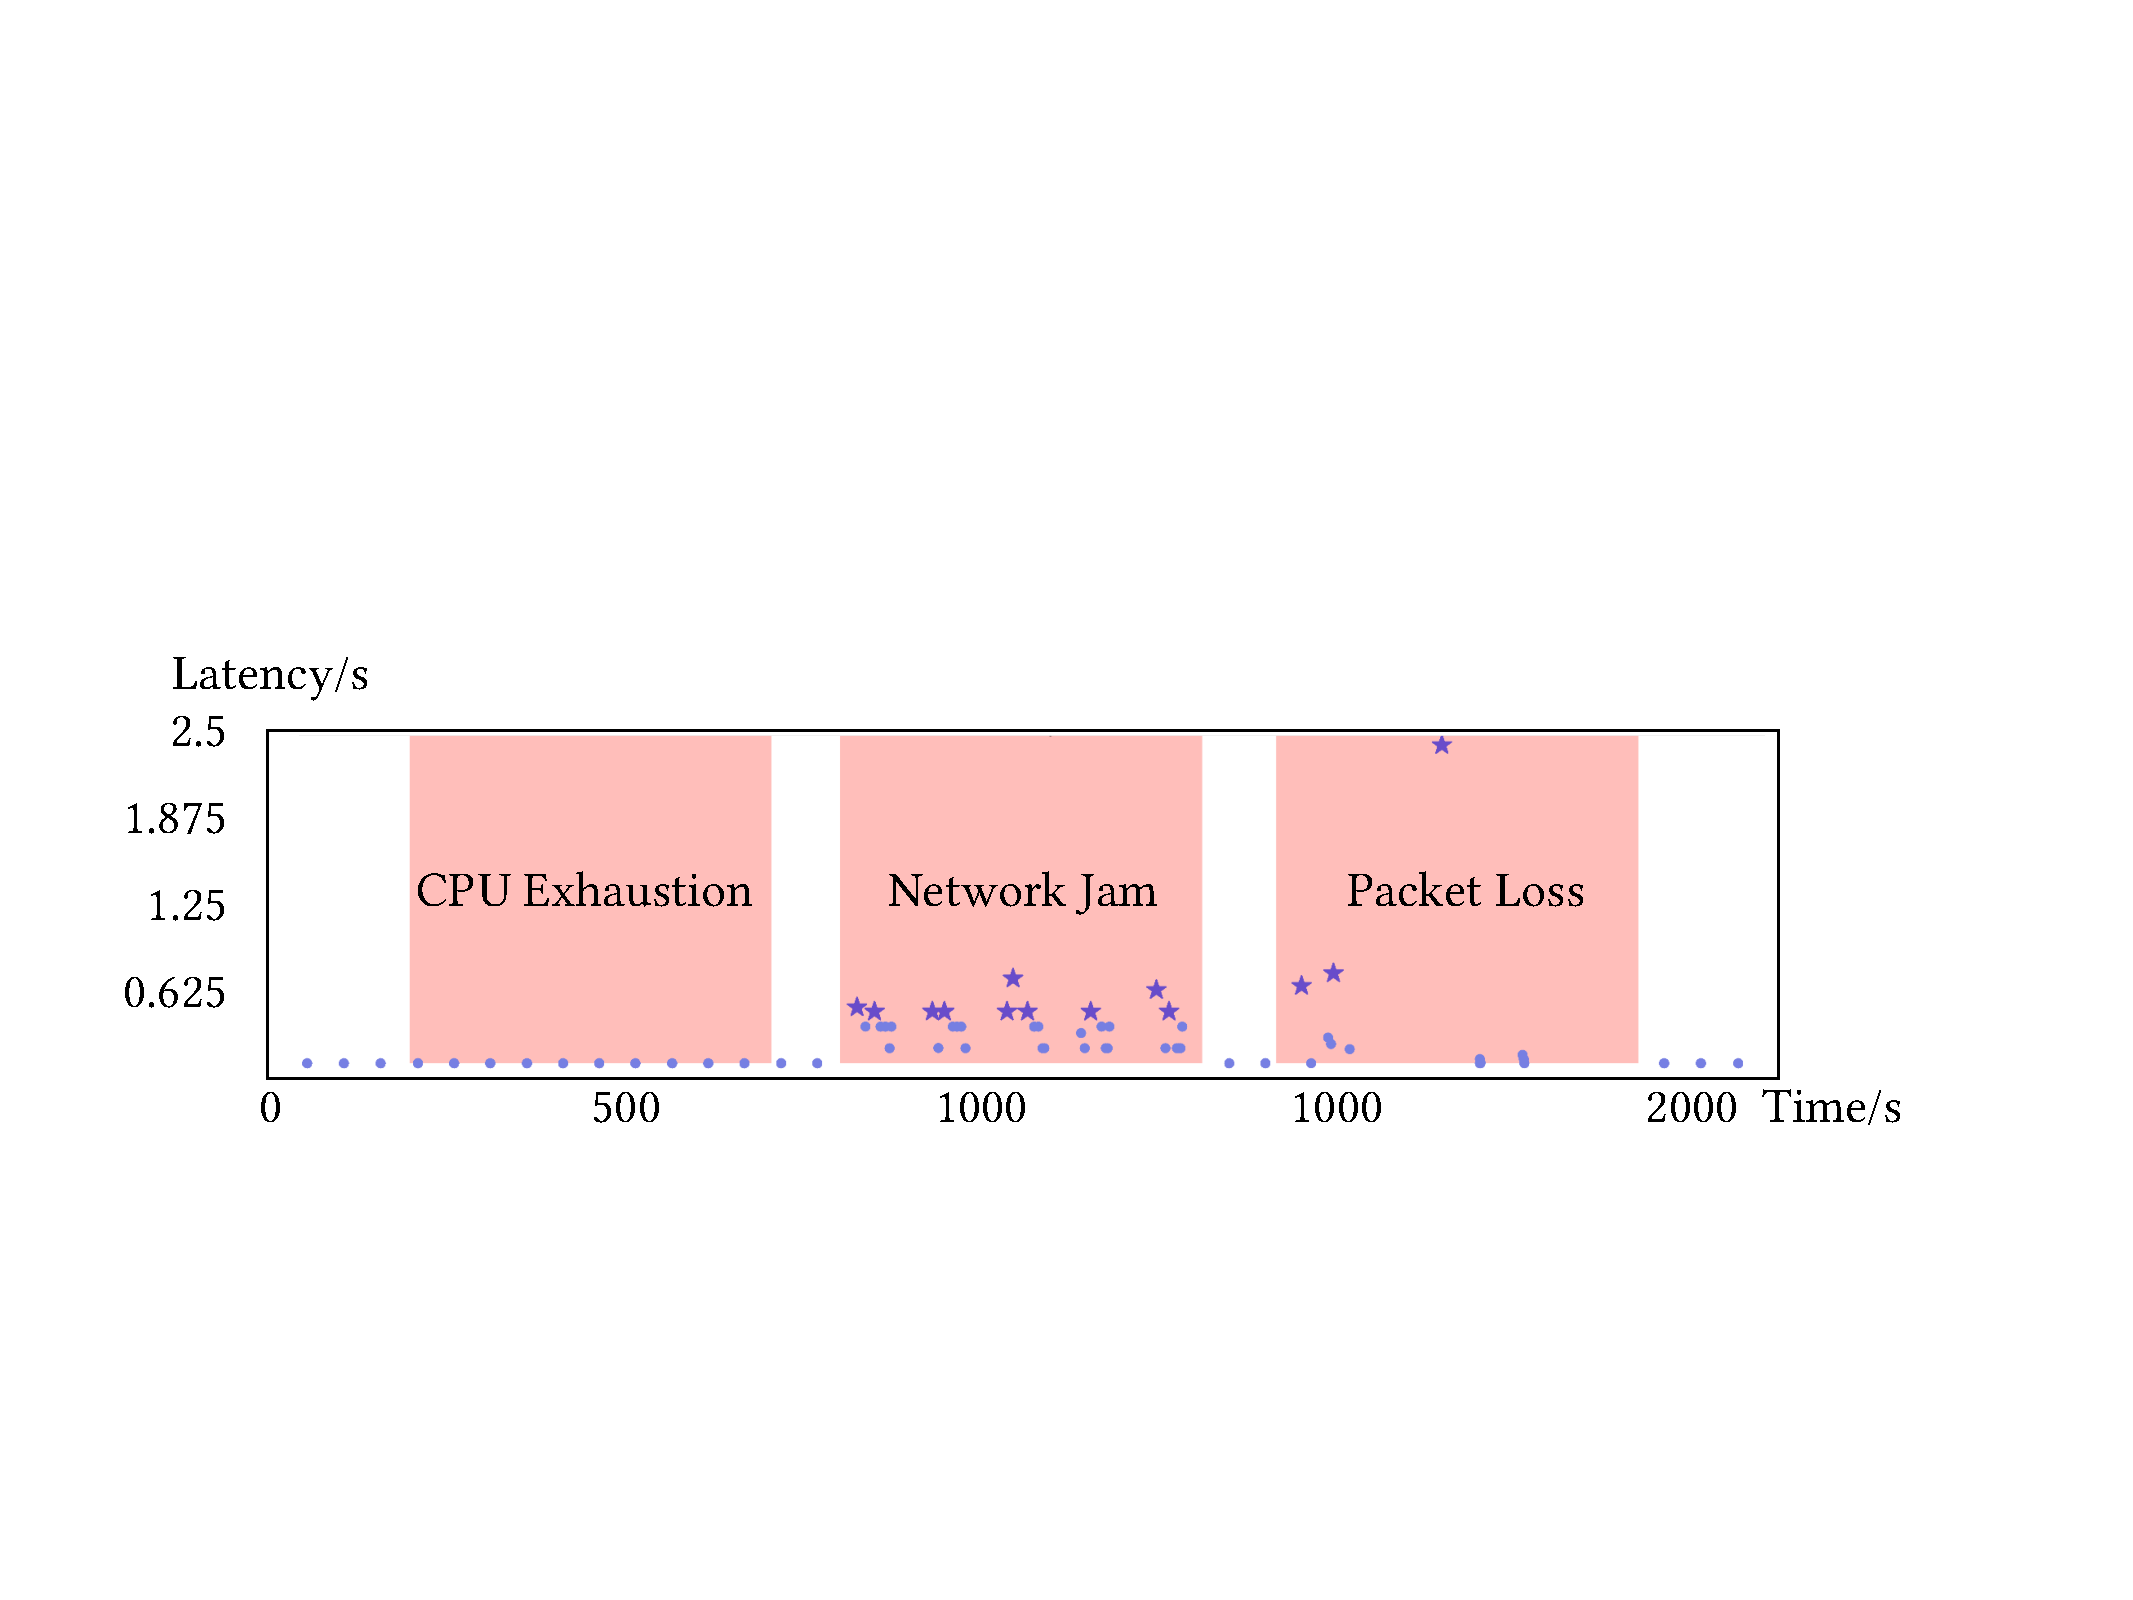
\includegraphics[width=0.97\linewidth]{figures/latency.pdf}
    \caption{Network-related faults incur obvious anomalies in latency of ``travel'', but the CPU exhaustion fault does not.}
    \label{fig:travel-latency}
\vspace{-0.1in}
\end{figure}

We also notice that \textit{system logs and KPIs provide valuable information manifesting anomalies in microservices.}

As for logs, we first parse all logs into events via Drain~\cite{Drain}, a popular log parser showing effectiveness in many studies~\cite{SurveyHe, reportZB}.
It is evident that some logs can report anomalies semantically by including keywords such as ``exception'', ``fail'', and ``errors''. The event ``Exception in monitor thread while connecting to server $<$\textit{*}$>$.'' can be a good example. 

Event occurrences can also manifest anomalies besides semantics. 
Take the event ``Route id: $<$\textit{*}$>$'' recorded by the microservice ``route'' as an example. This event occurs when the microservice completes the routing request.
Figure~\ref{fig:route-log} shows that when network-related faults are injected, the example event's occurrence experiences a sudden drop and remains at low values. The reason is that the routing invocations become less since the communication between ``route'' and its parent microservices (callers) is blocked.
This case further supports our intuition that system logs can provide clues about microservice anomalies.

\begin{figure}[htb]
    \centering
    \vspace{-0.1in}
    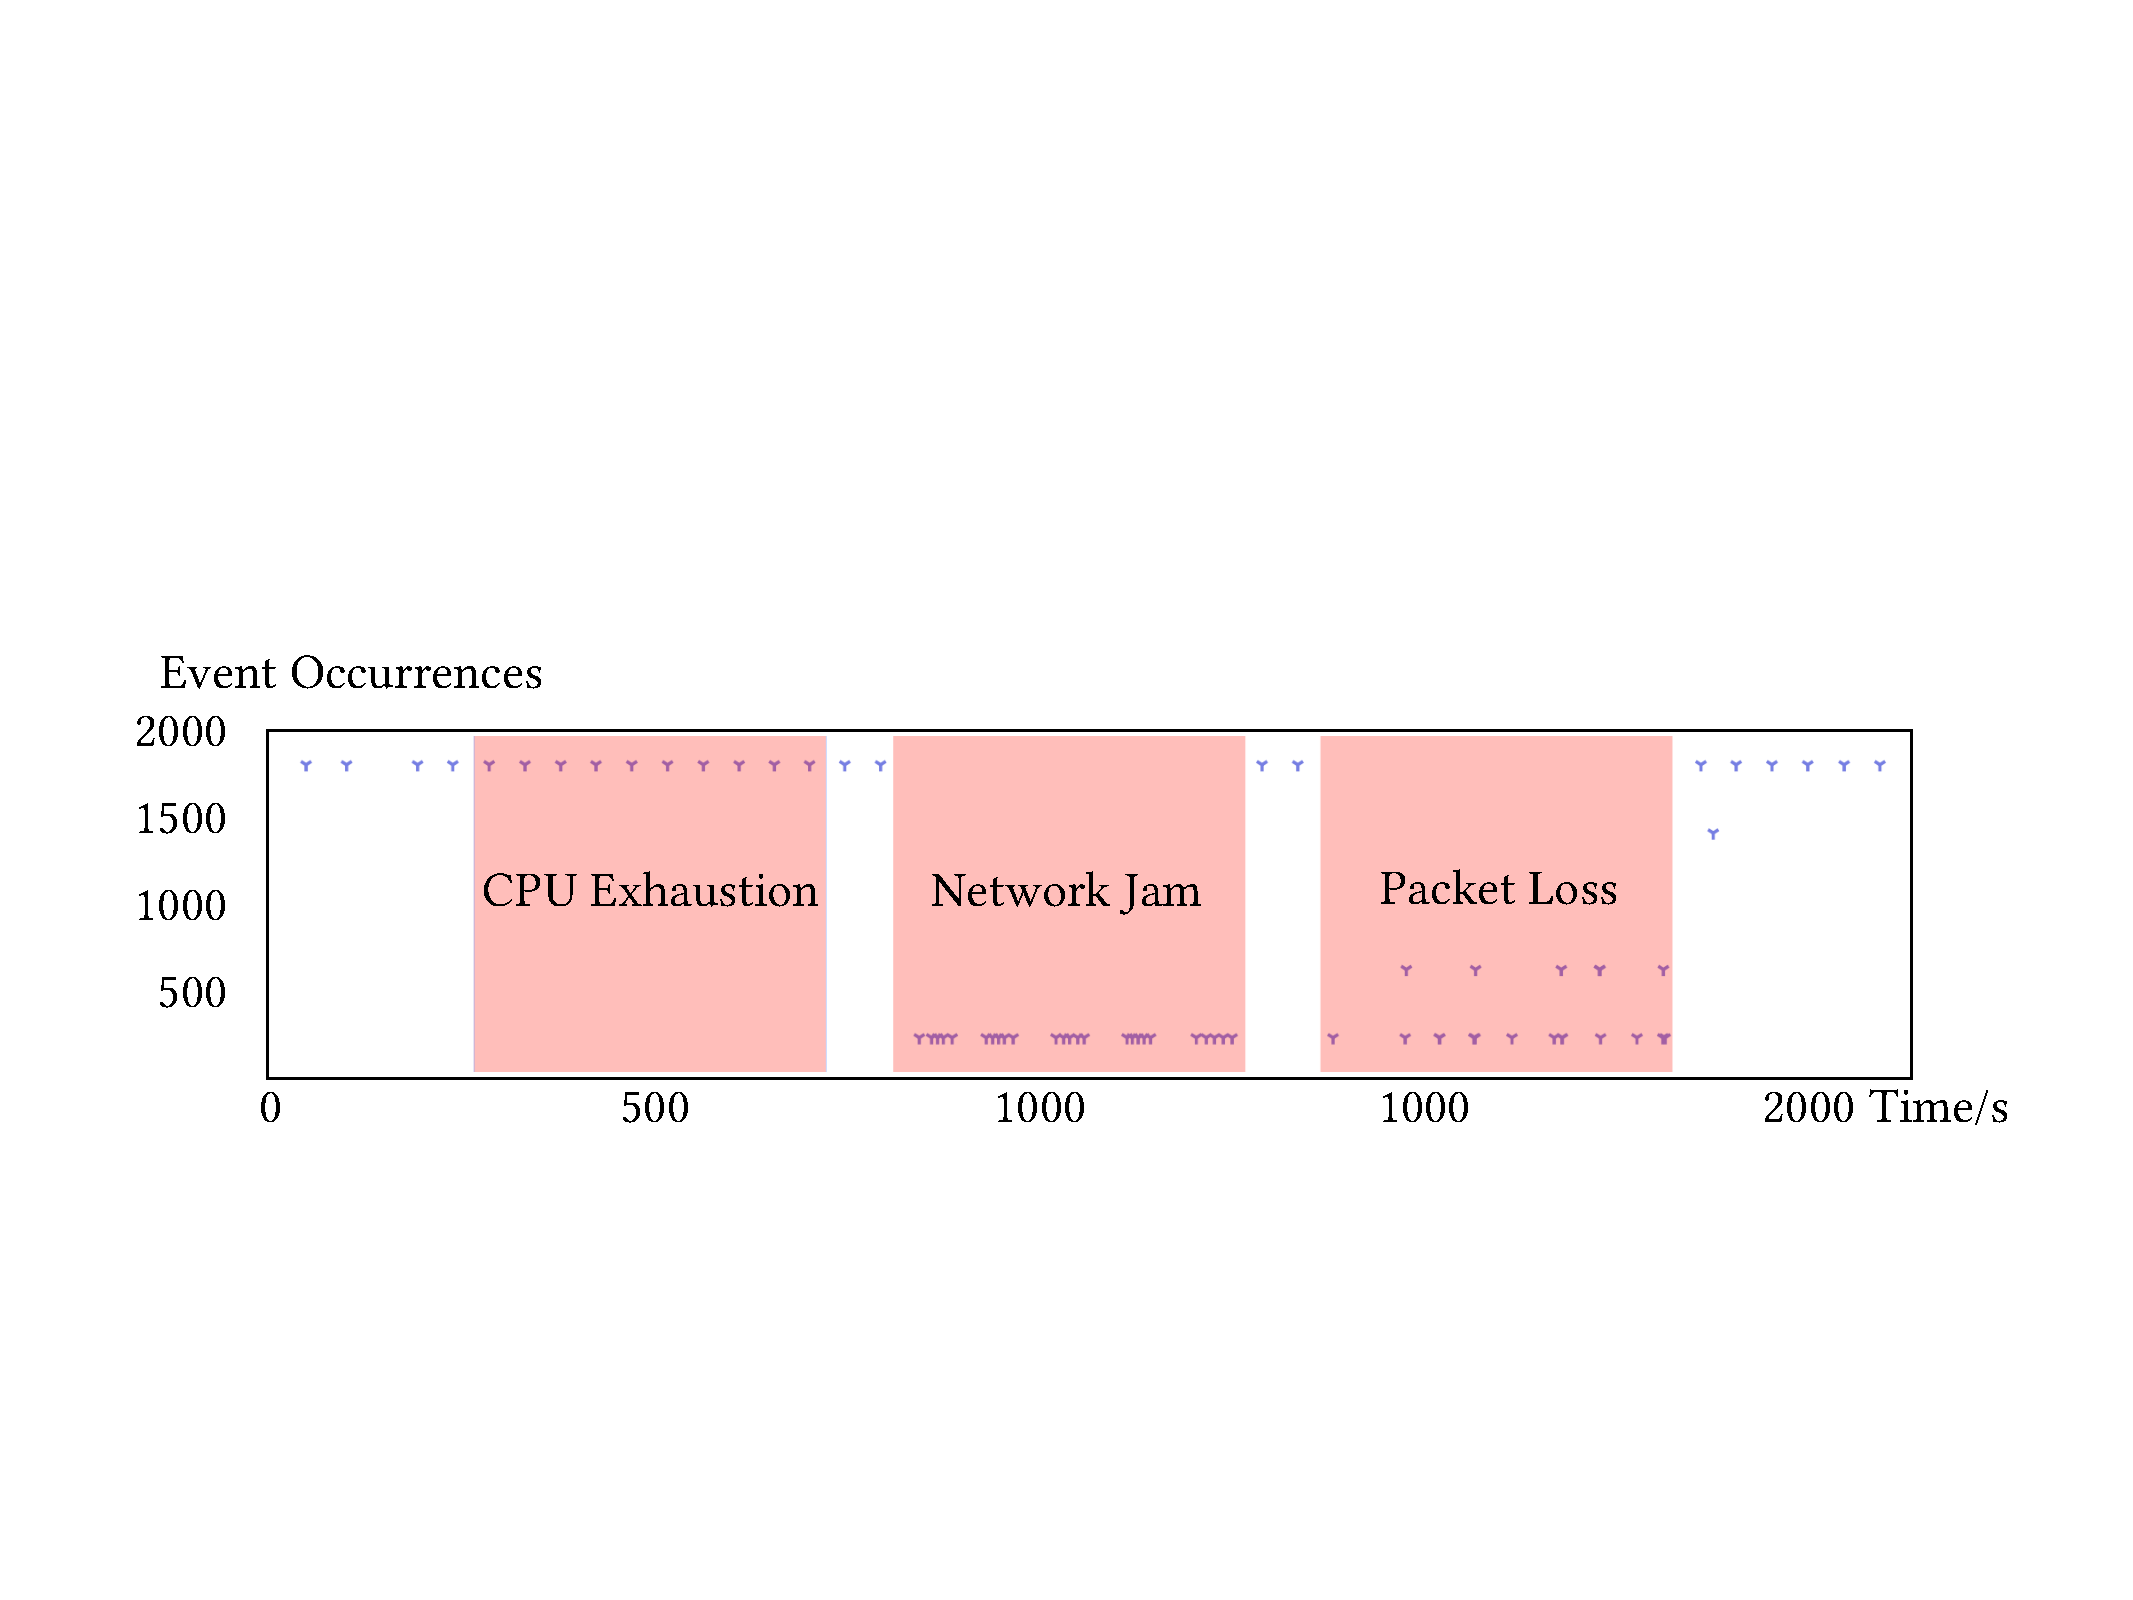
\includegraphics[width=0.95\linewidth]{figures/log.pdf}
    \caption{The occurrences of related logs can reflect issues such as poor communication.}
    \label{fig:route-log}
\vspace{-0.1in}
\end{figure}

KPIs are responsive to anomalies by continuously recording run-time information.
An example in Figure~\ref{fig:payment} gives a closer look, which displays ``total CPU usage'' of microservice ``payment'' during the period covering fault injections.
Clearly, ``total CPU usage'' responds to the fault CPU Exhaustion by showing irregular jitters and abnormally high values. This observation aligns with our a priori knowledge that KPIs provide an external view of a microservice's resource usage and performance. Their fine-grained information can well reflect anomalies, especially resource-related issues, which require detailed analysis.

\begin{figure}[htb]
    \centering
    \vspace{-0.1in}
    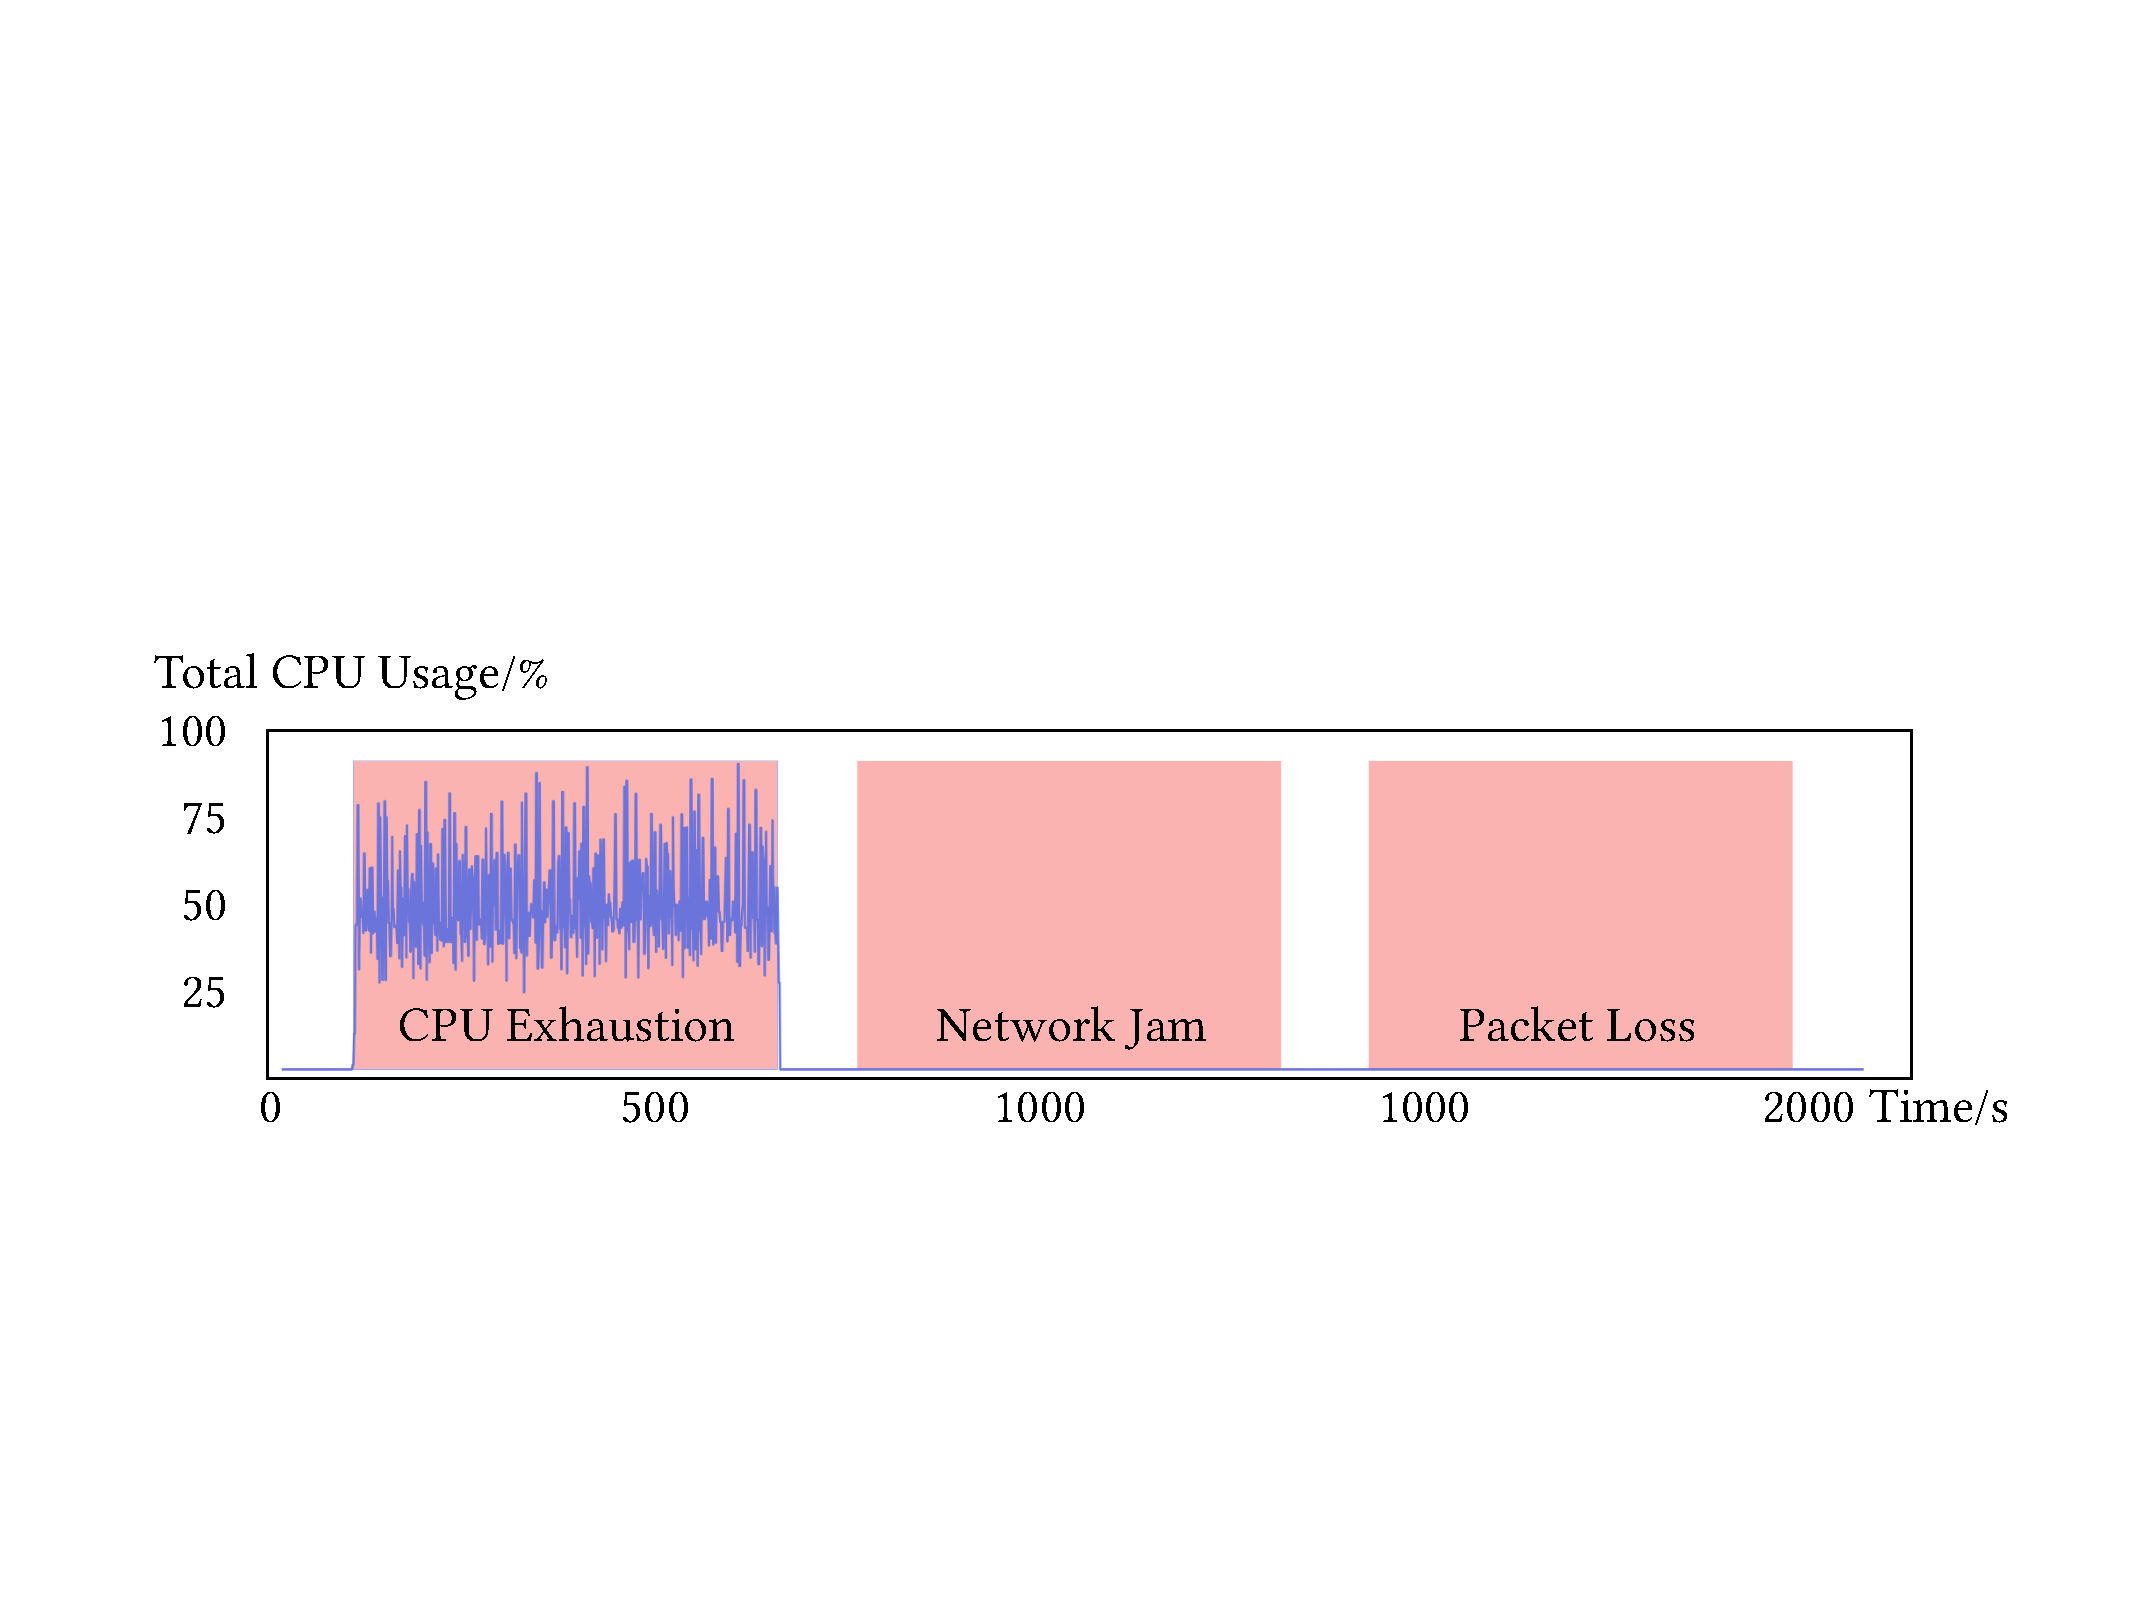
\includegraphics[width=0.95\linewidth]{figures/metric.pdf}
    \caption{A CPU exhaustion fault incurs abnormal jitters and high values in ``total CPU usage''.}
    \label{fig:payment}
\vspace{-0.1in}
\end{figure}

However, only using logs and KPIs is not sufficient since they are generated by each microservice individually at a local level. As the example shown in Figure~\ref{fig:dependency-graph} (\cref{sec:intro}), we need traces to obtain inter-service dependencies to analyze the anomaly propagation so as to draw a global picture of the system to locate the root cause.

\begin{mybox}
    Traces are informative yet not sufficient to reflect all anomalies. System logs and metrics provide valuable information manifesting anomalies by presenting abnormal patterns, so they can serve as additional information. 
\end{mybox}

\subsection{Can current anomaly detectors provide accurate results?}\label{sec:study:detection}
This section demonstrates that \textit{current detectors attached with localizers cannot deliver satisfying accuracy}. 

As far as we know, existing root cause localization approaches for microservices follow such a pipeline: 1) conduct anomaly detection and 2) if an anomaly is alarmed, then the localizer is triggered. That is, the anomaly detector and root cause localizer work separately.
Unfortunately, incorrect anomaly detection  results can exert a negative impact on the following root cause localization by introducing noisy labels.
To investigate whether current anomaly detectors are satisfactory for downstream localizers, we first summarize three main kinds of anomaly detection  approaches used in root cause localization papers. Note that since this paper targets root cause localization, the listed approaches are root cause localization-oriented anomaly detectors rather than sophisticated approaches for general anomaly detection.

\begin{itemize}[leftmargin=12pt, topsep=0pt]
\item N-sigma used in~\cite{MicroRank, MicroScope} computes the mean ($\mu$) and the standard deviation ($\sigma$) of historical fault-free data. If the maximum latency of the current observation window is larger than $\mu+n\cdot \sigma$, an alarm will be triggered, where $n$ is an empirical parameter.

\item Feature engineering + machine learning (FE+ML)~\cite{MicroHECL, AutoMAP} feeds manually derived features from traces into a machine learning-based model such as OC-SVM~\cite{MicroHECL} to detect anomalies in a one-class-classification manner. 

% The features are listed in Table~\ref{tab:features}.
\item SPOT~\cite{SPOT} is an advanced algorithm for time series anomaly detection based on the Extreme Value Theory. Recent root cause analysis studies~\cite{DyCause, MicroCause} have applied it for detecting anomalies.

\end{itemize}
\begin{table}[htbp]
\vspace{-0.1in}
\small
\centering
\caption{Comparison of Common Anomaly Detectors}
\begin{tabular}{cccc}
\toprule
& \textbf{N-sigma} & \textbf{FE+ML} & \textbf{SPOT} \\
\midrule
FOR & 0.632 & 0.830 & 0.638\\
FDR & 0.418 & 0.095 & 0\\
\#Infer/ms & 0.207 & 1.361 & 549.169\\
\bottomrule
\end{tabular}
\vspace{-0.1in}
\label{tab:fault-detection}
\end{table}

We conduct effectiveness measurement experiments based on our data on the three anomaly detectors following~\cite{MicroRank, MicroHECL, DyCause}, respectively. We focus on the false omission rate (\textit{FOR}$=\frac{FN}{FN+TN}$) and the false discovery rate (\textit{FDR}$=\frac{FP}{FP+TN}$), where
$TN$ is the number of successfully predicted normal samples; 
$FN$ is the number of undetected anomalies;
$FP$ is the number of normal samples incorrectly triggering alarms.
Besides, \#Infer/ms denotes the average inference time with the unit of microseconds.

Table~\ref{tab:fault-detection} lists the experimental results, demonstrating a large improvement space for these anomaly detectors. The high \textit{FOR} and \textit{FDR} indicate that the inputs of the root cause localizer contain lots of noisy labels, thereby substantially influencing localization performance.
We attribute this partly to the closed-world assumption relied on by these methods, that is, regarding normal but unseen data patterns as abnormal, thereby incorrectly forcing the downstream localizer to search for the ``inexistent'' root cause based on normal data.
Also, latency is insufficient to reveal all anomalies, as stated before, especially those that do not severely delay inter-service communications, represented by the high \textit{FOR}. 

In addition, complex methods (FE+ML and SPOT) have better effectiveness than N-sigma yet burden the troubleshooting process by introducing extra computation.
Since root cause localization requires anomaly detection first, the detector must be lightweight to mitigate the efficiency reduction. 
Even worse, these machine learning-based approaches require extra hyperparameter tuning, making the entire troubleshooting approach less practical.
\vspace{0.05in}
\begin{mybox}
    Root cause localization requires anomalous data detected by anomaly detectors, but current localization-oriented detectors either deliver unsatisfactory accuracy and introduce noisy data or reduce efficiency, making the following localization troublesome. 
\end{mybox}

In summary, these examples motivate us to design an end-to-end framework that integrates effective anomaly detection and root cause localization in microservices based on multi-source information, i.e., logs, KPIs, and traces.
Logs, KPIs, and latency in traces provide local information on intra-service behaviors, while invocation chains recorded in traces depict the interactions between microservices, thereby providing a global view of the system status.
This results in \name, the first work to enable jointly detecting anomalies and locating the root cause, all the while attacking the above-mentioned limitations by learning the microservice status concerning both intra- and inter-service properties from various types of data.
